\section{Arquitectura Kappa}

\subsection{Principios de Diseño}

La principal característica de esta arquitectura es su fuerte uso de un registro de eventos inmutable 
y ordenado cronológicamente que actúa como única fuente de verdad sobre los datos ingresados al sistema.

De esta manera, se logra unificar el procesamiento de datos en batch y streaming tratándolos como un flujo continuo de eventos, 
eliminando la dualidad de código y reduciendo la complejidad operativa.

El procesamiento de estos datos se realiza mediante motores de procesamiento de eventos que leen este registro, 
aplican transformaciones determinísticas 
y generan resultados derivados que pueden recomputarse en cualquier momento desde el inicio del log.

Este principio de reproducibilidad permite regenerar el estado completo del sistema cuando cambian los requisitos 
o algoritmos de procesamiento, sin necesidad de mantener rutas de código separadas.

Las vistas materializadas son otro principio fundamental, 
donde los resultados procesados se almacenan en sistemas optimizados para consultas, 
proporcionando acceso eficiente al estado actual sin necesidad de reprocesar todo el historial de eventos.

\subsection{Stack Tecnológico}

Para la capa de ingesta y transporte de datos, la Arquitectura Kappa implementa \textbf{Apache Kafka} como componente central, 
funcionando no solo como sistema de mensajería sino como la fuente única de verdad y almacén principal de eventos. 
En Kappa se configura Kafka con períodos de retención extendidos, 
aprovechando la capacidad de compactación de logs para mantener el historial completo de eventos mientras 
se optimiza el espacio de almacenamiento. 
Esto se logra agregando la capacidad de almacenamiento en capas, mediante la cual se pueden mantener los eventos
en Object Storage (utilizando \textbf{MinIO}), cuando pasa un tiempo definido de mantención en almacenamiento local.

El procesamiento de datos se realiza mediante \textbf{Apache Flink},
se despliega en un cluster con un nodo Job Manager y cinco nodos Task Manager; de forma de distribuir la carga de trabajo lo mejor posible.
En este caso, se define como punto de entrada un tópico de Kafka, para procesar los datos en tiempo real y
enviarlos a un nuevo topico y continuar con el procesamiento más adelante en la arquitectura.

En el último paso, se guarda el resultado del procesamiento en \textbf{Apache Doris}, un motor de análisis de datos
distribuido que permite realizar consultas SQL en tiempo real sobre grandes volúmenes de datos con una interfaz basada en MySQL.
Este componente permite escalar de forma diferente el acceso a los datos del procesamiento, 
siendo desplegado como un nodo frontend y tres nodos backend. 
Estos comparten el trabajo de procesamiento de consultas y almacenamiento de datos, 
mientras que el frontend se encarga de la distribución de las mismas. 
\subsection{Vista de Componentes}

\begin{figure}[h]
\centering
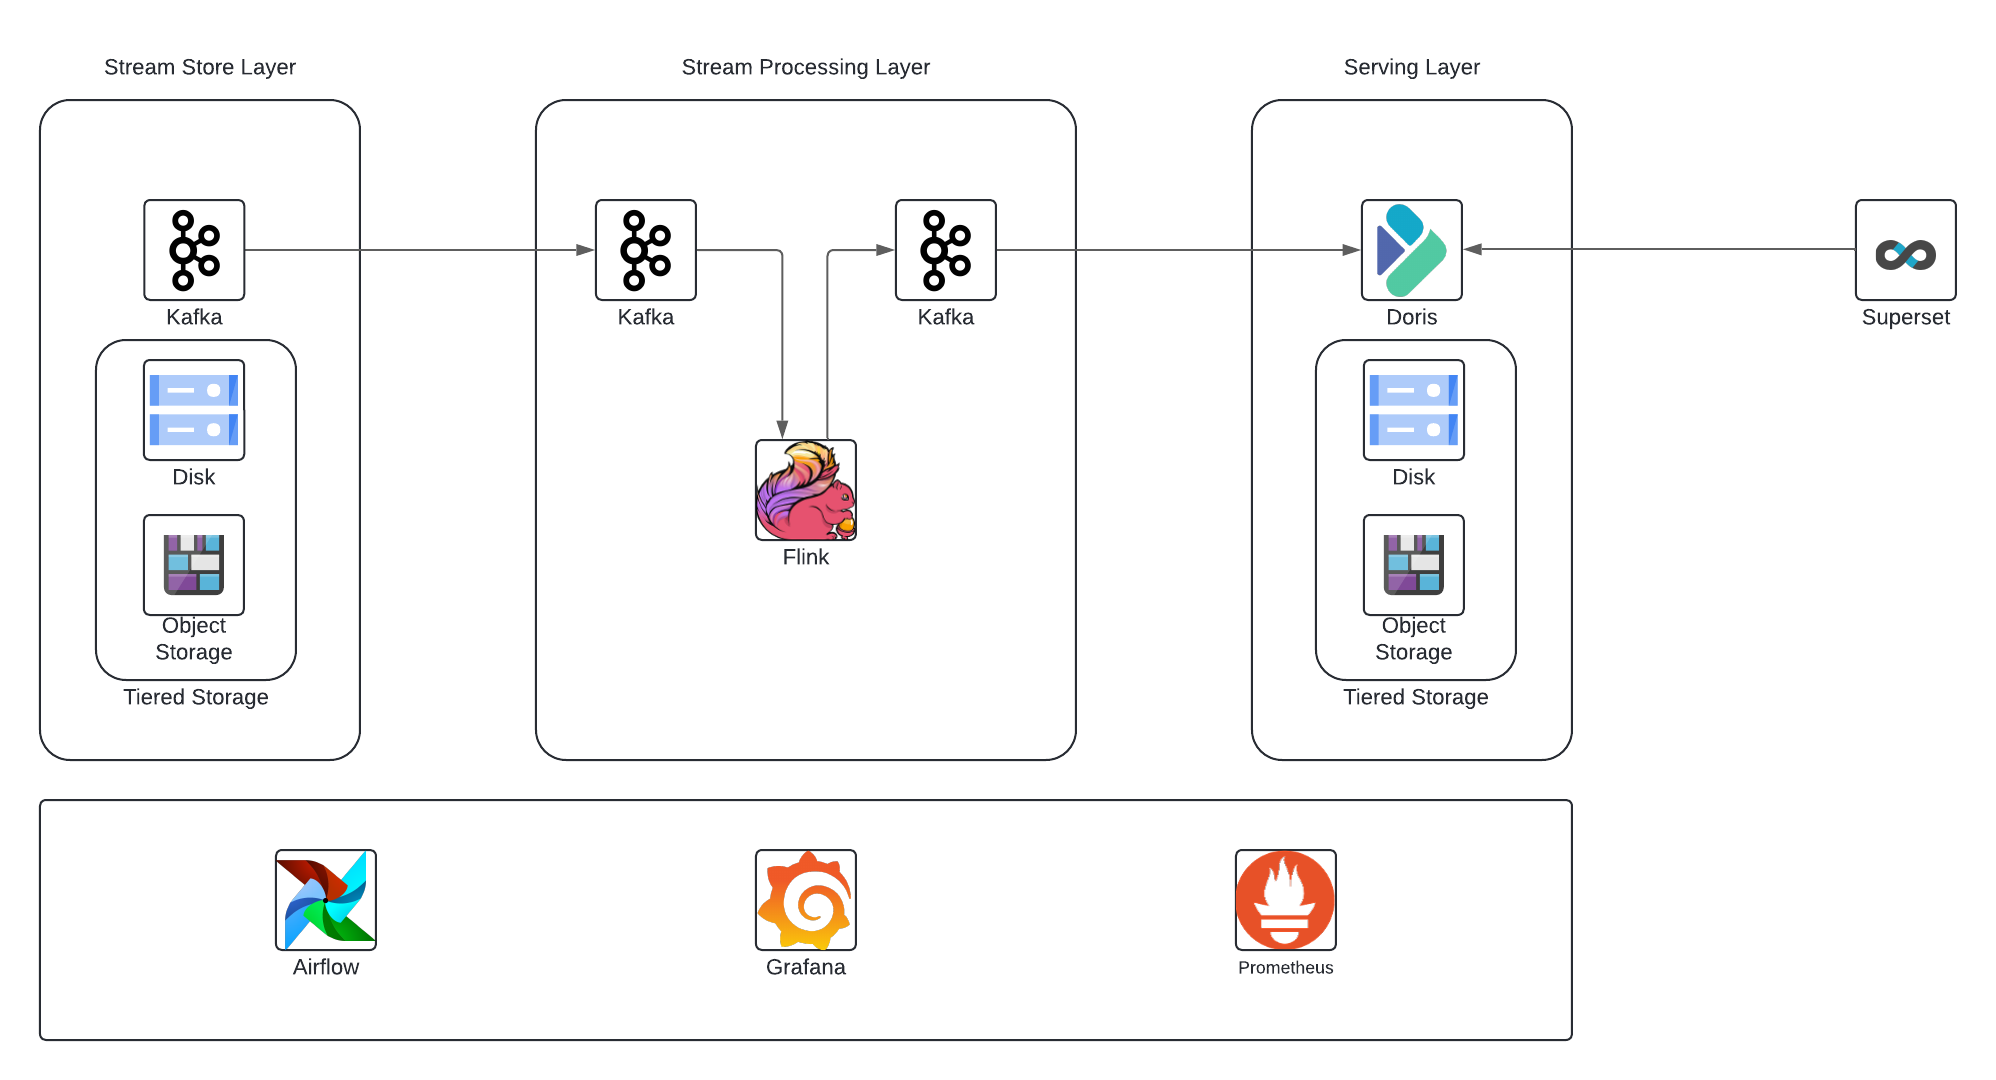
\includegraphics[width=1\textwidth]{desarrollo/Kappa.png}
\caption{Diagrama de la Arquitectura Kappa}
\label{fig:des_arquitectura_kappa}
\end{figure}

\subsection{Vista de Despliegue}

\subsection{Flujo de Procesamiento}
